\documentclass[a4paper,11pt]{article}
\usepackage[a4paper, margin=2.5cm]{geometry}

\usepackage[slovene]{babel}
\usepackage[utf8]{inputenc}
\usepackage[T1]{fontenc}

\usepackage{amsmath}
\usepackage{amsthm}
\usepackage{amssymb}
\usepackage{graphicx}
\usepackage{url}
\usepackage{booktabs}

{\theoremstyle{plain}
\newtheorem{izrek}{Izrek}
}

{\theoremstyle{definition}
\newtheorem{definicija}{Definicija}
}

\newcommand{\f}{\mathcal{F}}

\title{Brownovo gibanje}
\author{Matej Rojec}
\date{}

\begin{document}

\maketitle

Brownovo gibanje (več v \cite{karatzas1991brownian}) je intuitivno slučajen proces, % Sklic na knjigo
ki predstavlja naključno gibanje delcev v mediju.
    
% Slika: PerrinPlot2.pdf
% Napis pod sliko: 
% Reprodukcija slike iz Jean Baptiste Perrin, \emph{Mouvement brownien et réalité moléculaire}, Ann. de Chimie et de Physique (VIII) 18, 5-114, 1909
\begin{figure}[!ht]
    \centering
    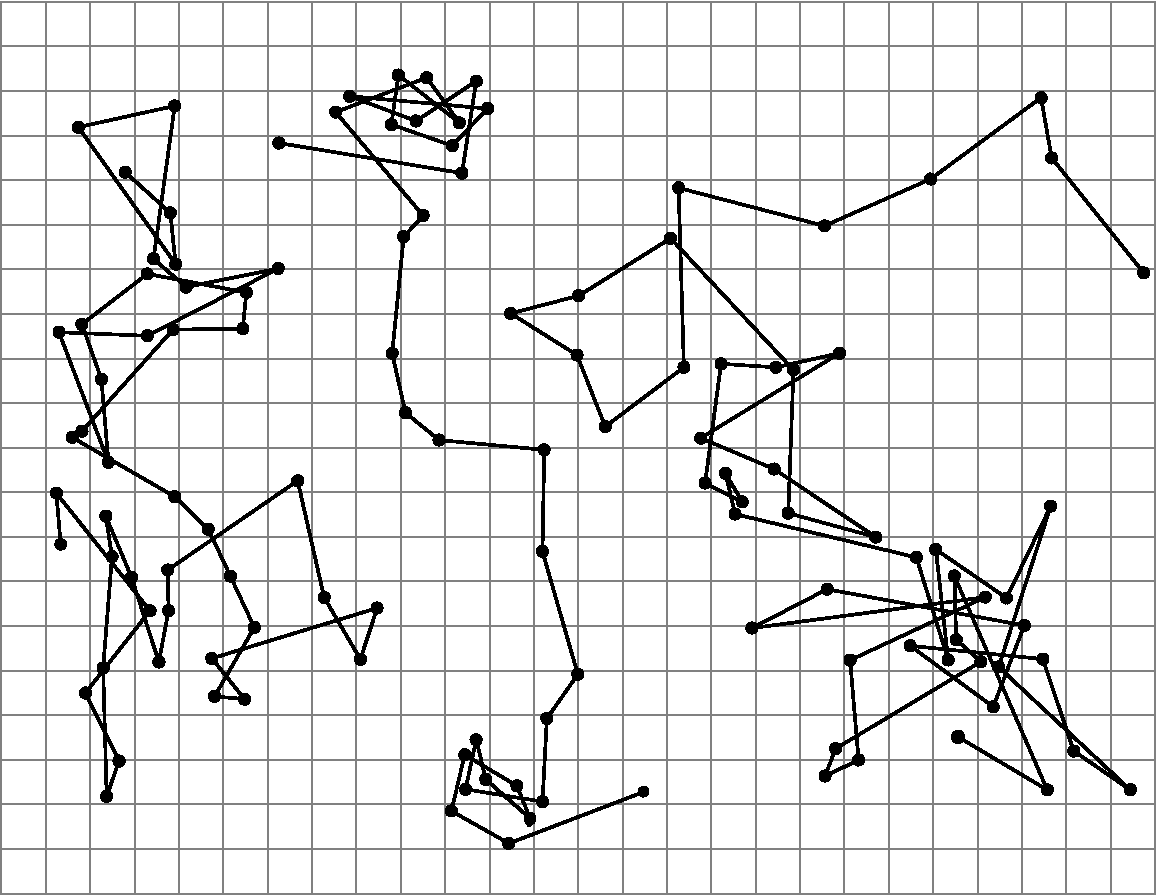
\includegraphics[scale=0.33]{PerrinPlot2.pdf}
    \caption{Reprodukcija slike iz Jean Baptiste Perrin, \emph{Mouvement brownien et réalité moléculaire}, Ann. de Chimie et de Physique (VIII) 18, 5-114, 1909}
    \label{fig:PerrinPlot2}
    \end{figure}


% Začetek definicije

\begin{definicija}
    Standardno Brownovo gibanje $\{B_t\}_{t \geq 0}$ je slučajen proces z naslednjimi lastnostmi: 
    \begin{enumerate}
        \item $B_0 = 0$.
        \item Prirastki $B_{t_n} - B_{t_{n-1}}, B_{t_{n-1}} - B_{t_{n-2}}, \ldots, B_2 - B_1, B_1 - B_0$ so neodvisne slučajne spremenljivke, za vsak $t_0 \leq t_1 \leq \cdots \leq t_{n-1} \leq t_n$.
        \item Za vsak $t \geq 0$ in $h > 0$ velja $B_{t+h} - B_t \sim \mathcal{N}(0, h)$.
        \item Funkcija $t \mapsto B_t$ je zvezna skoraj gotovo.
    \end{enumerate}

\end{definicija}
% Konec definicije

Preden zapišemo izrek, definirajmo še pojem časa ustavljanja.

% Začetek definicije

\begin{definicija}
    Slučajna spremenljivka $\tau$ na verjetnostnem prostoru $\Omega, \f, P$ z vrednostmi v $\mathbb{R} ^+$
    je \emph{čas ustavljanja glede} na filtracijo $(\f_t)_{t \in T}$ , če velja $\forall t \in T : \{\tau \leq t\} \in \f_t$.
\end{definicija}
% Konec definicije

Zdaj lahko zapišemo izrek \ref{thm:stopped_brownian}. % Sklic na izrek z oznako thm:stopped_brownian

% Začetek izreka

\begin{izrek}
    \label{thm:stopped_brownian}
    Naj bo $\{B_t\}_{t \geq 0}$ (standardno) Brownovo gibanje, $\tau$ čas ustavljanja glede na 
    $(\f_t)_{t\geq 0}$ in naj velja $P[\tau < \infty] = 1$.
    Potem je tudi proces:
    \[
    \hat{B} := \{B_{T+t} - B_T \mid t \geq 0\}
    \]
    (standardno) Brownovo gibanje in neodvisen od $\f_T$.
\end{izrek}
% Konec izreka

\bibliographystyle{plain}

\bibliography{knjiga}
    
\end{document}